\documentclass[svgnames]{beamer}

\usetheme{Madrid}
\usecolortheme{seahorse}
\usepackage{multirow}
\usepackage{caption}
\setbeamertemplate{navigation symbols}{}
\useinnertheme{rectangles}

\usepackage{appendixnumberbeamer}
\usepackage[ruled, vlined, longend]{algorithm2e}

\beamertemplatenavigationsymbolsempty
\usepackage[many]{tcolorbox}
\usepackage{color}
\usepackage{varwidth}
\usetikzlibrary{decorations.pathmorphing}
\usetikzlibrary{shadows}
\usetikzlibrary{svg.path}
\usepackage[absolute,overlay]{textpos}

\usepackage{listings}
\lstset {
  backgroundcolor=\color{white},
  basicstyle=\ttfamily\footnotesize,
  numbers=left,numberstyle=\tiny,numbersep=5pt,
  emph={proc, fun, let, send, consume, global, type, record, if, else,
    in, not, foldt, return, on, ordering, by, as, or },
  emphstyle={\bfseries},
  literate = {=>}{{\bf=>}}2
}
\usepackage{graphicx,accents,pinlabel}
%\useoutertheme{default}
%\useinnertheme{rounded}

\titlegraphic{
\begin{center}
\includegraphics[width=6cm]{poker_routes}%
\end{center}
}

\usepackage{tikz}
\usetikzlibrary{fadings,shapes.arrows,shadows}
\usetikzlibrary{shadows.blur}
\usetikzlibrary{shapes.symbols}
\usetikzlibrary{backgrounds}
\usetikzlibrary{arrows.meta}
\usetikzlibrary{shapes,snakes}
\usetikzlibrary{fit,calc,shadows}
\usetikzlibrary{arrows,shapes}
\setbeamercolor{section in head/foot}{bg=white, fg=black}
%\beamertemplateshadingbackground{black!10}{blue!15}
\makeatletter
\setbeamertemplate{footline}
{
  \leavevmode%
  \hbox{%
  \begin{beamercolorbox}[wd=.333333\paperwidth,ht=2.25ex,dp=1ex,center]{section in head/foot}%
    \usebeamerfont{author in head/foot}\insertshortauthor~~\beamer@ifempty{\insertshortinstitute}{}{}
  \end{beamercolorbox}%
  \begin{beamercolorbox}[wd=.333333\paperwidth,ht=2.25ex,dp=1ex,center]{section in head/foot}%
    \usebeamerfont{date in head/foot}\insertshortdate{}\hspace*{2em}
  \end{beamercolorbox}%
  \begin{beamercolorbox}[wd=.333333\paperwidth,ht=2.25ex,dp=1ex,right]{section in head/foot}%

    \insertframenumber{} / \inserttotalframenumber\hspace*{2ex} 
  \end{beamercolorbox}}%
  \vskip0pt%
}
\makeatother
\title{Mixed and time varying models for evolving complex networks}
\titlegraphic{
\begin{center}
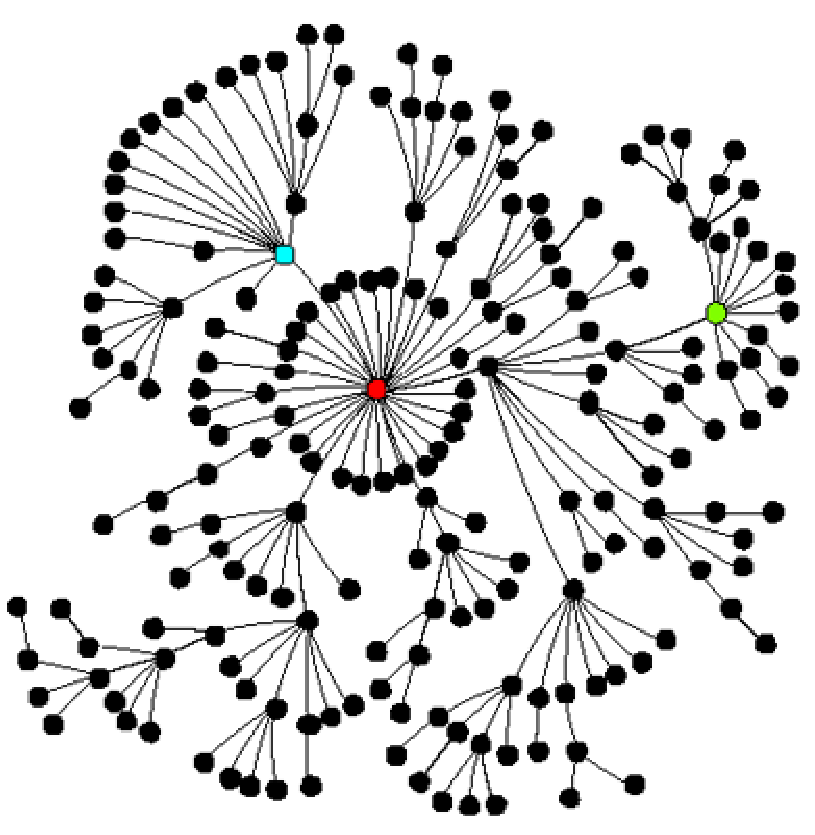
\includegraphics[width=3cm]{scale1}%
\end{center}
}

\author[Richard G. Clegg \& Naomi Arnold] {Richard G. Clegg (r.clegg@qmul.ac.uk) \\ 
Naomi Arnold (n.a.arnold@qmul.ac.uk) \\
Queen Mary University of London } 

\newcommand{\mr}{\mathbb{R}} %math R%
\newcommand{\mn}{\mathbb{N}} %math N%
\newcommand{\mz}{\mathbb{Z}} %math Z%
\newcommand{\bG}{\mathbf{G}}
\newcommand{\bg}{\mathbf{g}}
\newcommand{\btheta}{\mathbf{\theta}}
\newcommand{\var}[1]{\text{var}\left(#1\right)}
\newcommand{\Esym}{\text{E}}
\newcommand{\E}[1]{\Esym\left[#1\right]}
\newcommand{\Probsym}{\mathbb{P}}
\newcommand{\Prob}[1]{\Probsym\left[#1\right]}
\definecolor{burntorange}{cmyk}{0,0.52,1,0}
\tikzstyle{superpeers}=[draw,circle,burntorange, left color=\oran,
                       text=violet,minimum width=20pt]

\tikzstyle{big comment} = [draw, fill=blue!40, text=white, text width=8cm, minimum height=0.8cm, rounded corners, drop shadow, align=center]
\def\oran{orange!30}
\tikzstyle{vertex}=[circle,fill=black!25,minimum size=20pt,inner sep=0pt]
\tikzstyle{edge} = [draw,ultra thick,-]

\date[NetSci 3, Leeds]{3rd UK Network Science Workshop, Leeds 2019}

\begin{document}

\frame{

\begin{center}
\Huge{\inserttitle}


\vspace{0.2cm}

\inserttitlegraphic

\vspace{0.2cm}

\scriptsize{\insertauthor}

\vspace{0.2cm}

\scriptsize{\insertdate}

\vspace{0.2cm}

\tiny{(Prepared using \LaTeX \;and beamer.)}
\end{center}
}


\frame{
\frametitle{Problem statement}
\begin{itemize}
\item Evolving networks (graphs/topologies) 
are an important topic for research.
\item Want to describe and understand processes which govern
evolution.
\item Motivating example models of similar form to Barab\'asi--Albert (1999)
\end{itemize}
\begin{block}{Problem statement (vague)}
\begin{itemize}
\item Want to grow networks with the \alert{same properties} as
real networks.
\item Want to be able to describe the \alert{evolution} 
of the real network.
\item Want to be able to compare rival theories about the evolution.
\end{itemize}
\end{block}
}
\tikzstyle{edge} = [draw,ultra thick,-]
\frame{
\frametitle{Models of graphs -- Erd\H{o}s--R\'{e}nyi (1959)}
\begin{itemize}
\item Perhaps the most famous graph model -- nodes are added at random.
\item With probabilty $p$ two nodes are linked.
\item Pro: Easy to reason about.
\item Con: Not a good model for most real-world networks.  
\item Con: Doesn't say anything about order edges appear.
\end{itemize}
\centering{
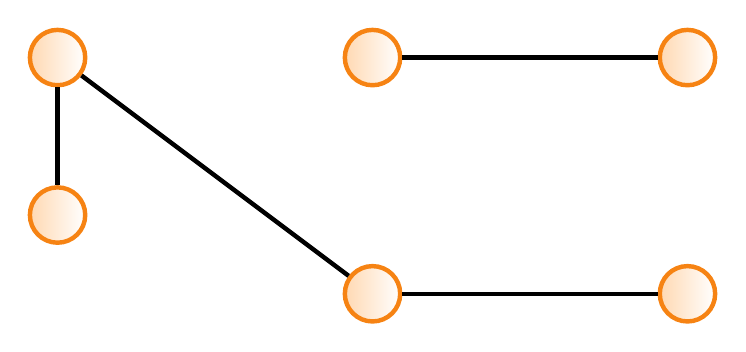
\begin{tikzpicture}[remember picture,auto, ultra thick]
  % Place super peers and connect them
  \foreach \place/\name in {{(0,-1)/a}, {(4,-1)/b}, {(4,2)/c}, {(0,2)/d},
           {(-4,0)/e}, {(-4,2)/f}}
    \node[superpeers] (\name) at \place {};
  \path <2-> (f) edge (e);
  \path <3-> (d) edge (c);
  \path <4-> (a) edge (b);
  \path <5-> (a) edge (f);
\end{tikzpicture}
}
}


\frame{
\frametitle{Models of graphs -- Scale-free Barab\'asi--Albert (1999)}
\begin{block}{Scale free networks}
A scale free network is one where the degree distribution
follows a power law -- $\Prob{\text{deg} = i} \sim i^{-\alpha}$.  
\end{block}
Scale free networks said to include:
\begin{itemize}
\item Internet Autonomous System (AS) graph [Faloutsos x 3 INFCOM 1999],
\item hyperlinks in web pages / wikipedia,
\item co-authorship/citation networks, and other social networks,
\item biological networks (protein networks).
\end{itemize}
\begin{block}{Preferential attachment}
Probability of attach to node $i$  proportional to node degree $d_i$.  That is  $p_i \sim 
d_i$. 
Leads to scale free network (Barab\'asi--Albert [Science 1999]).
\end{block}
}

\frame{
\frametitle{Many many network models exist}
\begin{itemize}
\item Generalised Linear Preference (GLP model) [FIX ME -- correct ref] 
\begin{itemize}
\item Probability of attachment to $i$ is degree $d_i$ modified by power $p_i \sim  d_i^ {\alpha}$ -- $\alpha$ is tunable parameter.
\end{itemize}
\item Positive Feedback Preference (PFP model) [Zhou--Mondrag\'on Phys Rev E 2004] (targetted at the Internet)
\begin{itemize}
\item Prob. of connecting to $i$ is 
$p_i \sim 
d_i^ {(1 - \delta \log_{10} d_i)}$ where
$\delta$ is a tunable parameter.
\end{itemize}
\item Jackson--Rogers [American Econ Rev 2007] (targetted at social networks)
\begin{itemize}
\item (Simplified explanation).  Pick $r$ nodes completely at random.  Pick $q$ nodes that neighbour these $r$ nodes.  $q$ and $r$ are tunable parameters.
\end{itemize}
\item Many others: Stochastic block models, exponential random graphs, Waxman model, Subgraph generation model, Statistical exponential random graphs.
\end{itemize}
}

\subsection{Problems arising}

\frame{
\frametitle{The ``basket of statistics" approach}

\begin{itemize}
\item Which model is ``best"?  How do we tune parameters?
\item Define the current approach the ``basket of statistics" method.
\begin{enumerate}
\item Select several statistics which can be measured on net snapshot.
\item Use test model to grow test network (same size as real network).
\item Compare the ``basket of statistics" on real and test.
\end{enumerate}
\item New statistics motivate new models -- but what if not all stats match?
\end{itemize}

Topology modelling appears to be progressing in the following manner:
\begin{enumerate}
\item Analyse snapshot of graph (topology) of interest.
\item Find some statistic  the current
model does not replicate (add this to ``basket").
\item Create a new model which replicates the new statistic without
affecting old ones.
\item Test using the above procedure. 
\end{enumerate}

}


\frame{
\frametitle{Refined problem statement}
\begin{itemize}
\item Let $G(t)$ be a time evolving graph which evolves according
to some probabilistic process.
\item Let $\bG= (G_i, G_{i+1}, \ldots, G_{i+n})$ be random variables
representing this process observed at discrete times.
\item Let $\bg=(g_i, g_{i+1}, \ldots, g_{i+n})$ be a set of observations
of $\bG$.
\end{itemize}
\begin{block}{Problem statement --- more precise}
Given observations of a graph $\bg$ want to:
\begin{itemize}
\item Create models which formally specifies $\Prob{G_{t+1} = g_{t+1} | 
G_t=g_t,\ldots}$.
\item Likelihood is a term in statistics it measures the probability a given data set arose if an explanatory model is true.
\item Measure the likelihood of such a model producing $\bg$.
\item Automatically test many such models.
\end{itemize}
\end{block}
}

\section{FETA}

\subsection{FETA approach}
\frame{
\frametitle{FETA approach}
\begin{center}
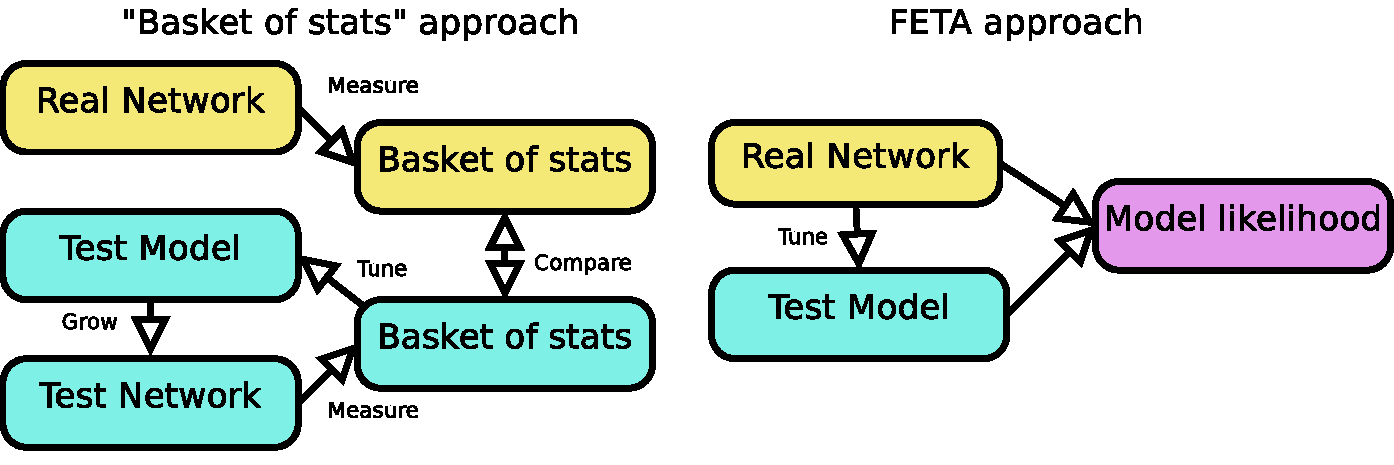
\includegraphics[width=10cm]{feta_process}
\end{center}
}

\subsection{A probabilistic model of graph evolution}
\frame{
\frametitle{A probabilistic model of graph evolution}
\begin{itemize}
\item Creating a parameterised model $M(\btheta)$ of $\Prob{G_{t+1} = g_{t+1} | 
G_t=g_t,\ldots}$.
is not straightforward.
\item This is not like normal stochastic process.  The dimensionality
of $G(t)$ changes over time.
\item Could transform to some multi-dimensional process with
dimension highest dimension graph will achieve (nasty solution).
\item Also want a solution which is compatible with existing research
in field (can test existing research methods).
\end{itemize}
}


\frame{
\frametitle{The FETA model structure}
\begin{block}{Operation model}
\begin{itemize}
\item Process to select an operation on the network.
\item Could be: \alert{add node}, 
\alert{add edge}, 
\alert{remove node} and so on.
\end{itemize}
\end{block}

\begin{block}{Object model}
\begin{itemize}
\item Process selects which nodes/edges are involved in operation
selected by operation model.
\item Probabilities are assigned to nodes and potential
edges for random selection.
\item Edges selected by assigning probabilities
to node pairs.
\item Object model is main focus of this presentation.
\end{itemize}
\end{block}
}

\frame{
\frametitle{FETA Model -- operations model example}
\begin{itemize}
\item Results reported here operation model can select from:
\begin{enumerate}
\item $\text{NewNodes}(n,m)$ Create a new node and connect it to 
$n$ new nodes and $m$ existing nodes.
\item $\text{NewLinks}(n)$ Select an existing node and connect it 
to $n$ existing nodes.
\item $\text{NewClique}(n,m)$ Create a clique between $n$ new nodes
and $m$ existing nodes.
\end{enumerate}
\item Example: Original preferential attachment model is:
$\text{NewNodes}(0,3)$.
\item Graph evolution is broken down into the addition of cliques,
new nodes and links between existing nodes.  (There is some ambiguity here).
\item The full operations model gives the probability of each operation
(with parameters) at each time step.
\item More focus needed on the operations model.  Here it is just
``copied" for real data.
\end{itemize}
}

\frame{
\frametitle{Importance of operations model}
\begin{center}
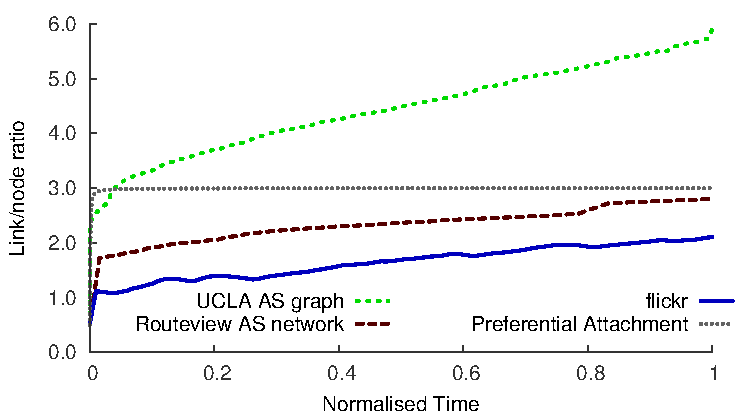
\includegraphics[width=10cm]{link_node_evolve}
\end{center}
}

\subsection{Object Model evaluation}

\frame{
\frametitle{Object model examples}
\begin{itemize}
\item For simplicity consider graphs which evolve using only the 
$\text{NewNode}(0,1)$ operation -- a new node is created and connects
to one existing node.
\item Some function which maps all possible choices
(of node or link) to a probability.
\item For example the Preferential Attachment model is
$p_i = d_i / k$ where:
\begin{itemize}
\item $p_i$ is the probability of choosing node $i$.
\item $d_i$ is the degree of node $i$.
\item $k$ is a normalising constant such that $\sum_i p_i = 1$.
\end{itemize}
\item The PFP model is $p_i = d_i^{1+\delta \log_{10} (d_i)}/k$
where $\delta$ is a parameter.
\end{itemize}
}

\subsection{From model to likelihood}

\frame{
\frametitle{The likelihood of FETA model}
\begin{itemize}
\item Let $M(\btheta)$ be a parameterised FETA model which
assigns probabilities to operations and object models with
some parameters $\btheta$.
\item Define $f_{i,M(\btheta)}(g_i)= \Prob{G_{i}=g_i| M(\btheta), G_{i-1}=g_{i-1}, 
G_{i-2}=g_{i-2}, \ldots}$
\item For convenience just write  $f_{i}(g_i)$
\item Then the likelihood of the model $M(\btheta)$ given the
observations $\bg$ (from $i$ to $i+n$)
is
$L(M(\btheta) | \bg ) = \prod_{k=i+1}^{k=i+n} f_k(g_k)$.
\item This likelihood defines how likely the model is given
the observations (or conversely, how probable the observations given
the model).
\item It is the ability to assign a true likelihood to the
graph evolution which is key to the FETA process.
\end{itemize}
}

\frame{
\frametitle{Building object models from components}
\begin{itemize}
\item Three possible object models have been introduced already.
\begin{enumerate}
\item $M_0$ -- all nodes equal.
\item $M_d$ -- preferential attachment (nodes weighted by degree).
\item $M_p(\delta)$ -- PFP model $\delta$ is parameter.
\end{enumerate}
\item How about mixture models?
\item $M= \beta_1 M_0 + \beta_2 M_d$ (nodes sometimes chosen randomly, 
sometimes by degree) -- $0 < \beta_1 < 1$ and $\beta_1+\beta_2= 1$.
\item On the positive site, a larger family of explanations, on the negative,
more parameterisation.
\end{itemize}
}

\frame{
\frametitle{Object model components}
Throughout $k$ is a normalising constant such that $\sum_i p_i = 1$
for all nodes considered.  
$p_i$ is the probability of picking node
$i$ (at the stage being considered).

FIXME -- use only models in this presentation
\begin{itemize}
\item Random model $M_0 \quad p_i = 1/k$.
\item Preferential attachment $M_d \quad p_i = d_i /k$.
\item PFP $M_p(\delta) \quad p_i = d_i^{1+\delta \log_{10} (d_i)}/k$  where $\delta$ is a parameter.
\item Degree power $M_d(\alpha) \quad p_i = d_i^{\alpha}/k$ where $\alpha$ is a parameter.
\item Triangle model $M_t \quad p_i =  t_i/k$ where $t_i$ is the triangle count of node $i$.
\end{itemize}
}

\frame{
\frametitle{A GLM approach to optimise $\beta$ parameters}
\begin{itemize}
\item Want to automatically fit $\beta_i$ in models of
form $M= \beta_1 M_1 + \beta_2 M_2 + \cdots$.
\item Functional form looks temptingly like a generalised linear model.
\item Let $p_{i,j}$ be the probability model assigns to node $i$ 
at step $j$.
\item Cannot fit to $p_{i,j}$ at each stage because probability is
not directly measureable.
\item Instead all we know is whether node $i$ was actually selected
or not at stage $t$.
\item Let $I_{i,j}$ be
an indicator variable such that $I_{i,j}$ is one if node $i$ was
chosen for choice $j$ and zero otherwise.
\item By definition $\E{I_{i,j}} =  p_{i,j}$.
\item Therefore, we fit models of the form
$I_{i,j} = \beta_1 M_1 + \beta_2 M_2 + \cdots$.
\item Obviously many models of this form can be tried.  Statistical
significance will reject unnecessary variables.
\end{itemize}
}


\section {Testing FETA}

\subsection{Artificial tests}

\frame{
\frametitle{Artificial tests}
\begin{itemize}
\item Perhaps the most convincing test of such a model is its ability to
recover parameters from a known model.
\item Build a model with known $M(\btheta)$.  Assume a model structure,
try to recover $\btheta$.
\item Two types of parameter -- $\btheta_{\cdot}$ parameters can be recovered
using Generalised Linear Model fitting.
\item Other (non-linear) parameters can be found from ``parameter sweeps" 
(assessing the likelihood for many values of that parameter).
\end{itemize}
}

\frame{
\frametitle{Sweep one parameter (10,000 link network)}
\centering{
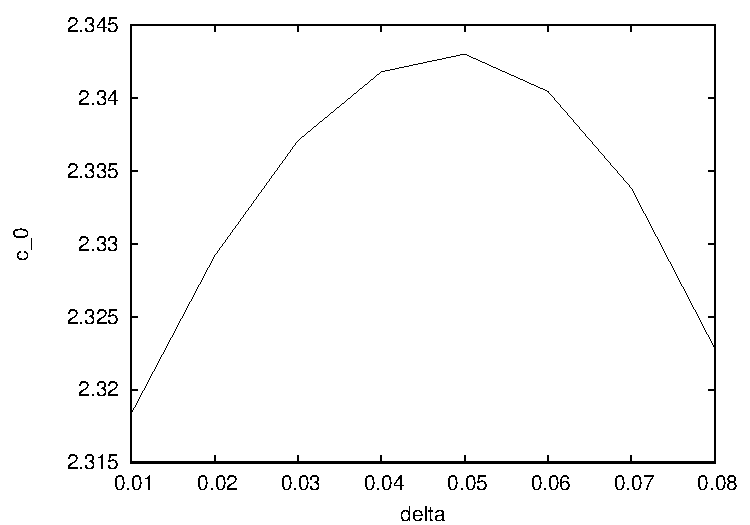
\includegraphics[width=10cm]{deltasweep} \\
}
PFP model $M= M_d(0.05)$.  Correct answer is $\delta = 0.05$.
}

\frame{
\frametitle{Sweep two parameters (10,000 link network)}
\centering{
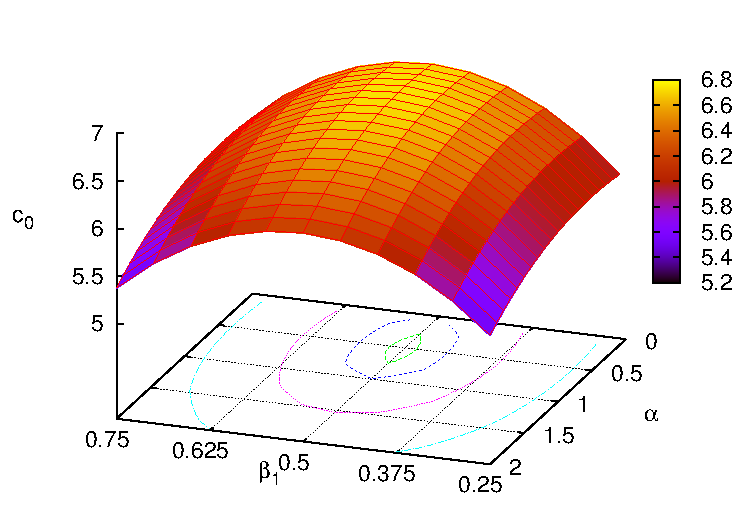
\includegraphics[width=8cm]{art1_data} \\
}
Correct model $M = 0.5 M_2 + 0.5 M_d(0.5)$
fitted $M= \beta_1 M_2 + (1-\beta_1) M_d(\alpha)$.
}

\frame{
\frametitle{Sweep two parameters (10,000 link network)}
\begin{center}
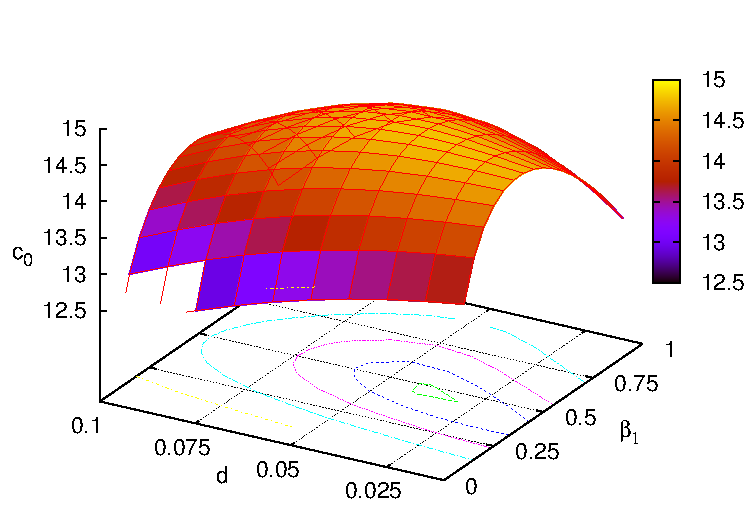
\includegraphics[width=8cm]{art2_data} \\
Correct model $M = 0.5M_p(0.05)+0.5M_t$ fitted 
$M= \beta_1 M_p(d)+(1- \beta_1)M_t$ 
\end{center}
}


\section{Conclusions}
\subsection{Conclusions}

\frame{
\frametitle{Conclusions}
\begin{itemize}
\item The likelihood parameters and the null model here provide 
a rigorous way to assess a potential dynamic model of network evolution.
\item The likelihood is reflected in improved performance on replicating
network statistics.
\item The advantages of this framework are several:
\begin{enumerate}
\item Assesses the dynamic history of the data not statistics of
a snapshot.
\item Single statistically rigorous estimate of model
likelihood.
\item Quicker than growing a network and testing
statistics (using same codebase).
\end{enumerate}
\item An exciting new way to test theories about topologies
if you have the data for it.
\end{itemize}
}

\frame{
\frametitle{Further work}
\begin{itemize}
\item Ongoing work -- lots still to do.
\item Software and data freely available -- please email 
{\tt n.a.arnold@qmul.ac.uk}
\item Code and data: 
{\tt https://github.com/narnolddd/FETA3}
\end{itemize}
}

\end{document}
